\chapter{Preliminaries and Related Work}\label{preliminaries}

\section{Fixed Topology}\label{flocking}

\subsection{Second-Order System}

Bird flocking or distributed behavior model was first studied in~\cite{Reynolds1987} to animate the aggregate motion of birds in computer simulation. Based on~\cite{Reynolds1987} and observations, a discrete time model (\ref{eq:vicsek}) and the correlation between flock coherence and particle density have been discussed in~\cite{Vicsek1995}. In this model, each particle has a constant velocity, while its direction is determined by ${\langle\theta(t)\rangle}_r$, which is the average direction of the neighboring particles within radius $r$, with $\Delta\theta$ representing the random noise. To clarify the notation, we identify the set of $k$ agents as $V=\{1,...,k\}$ and $x_{ij}=x_i-x_j$, where $x_i$ or $x_i(t)$ and $v_i$ or $v_i(t)\in\mathbb{R}^n$ represent the position and velocity of agent $i$ at time $t$ respectively. Unless otherwise noted, we assume the initial positions of the agents are distinct that $x_i(0)\neq x_j(0)$ for $i, j\in V$.

\begin{equation}\label{eq:vicsek}
\begin{aligned}
x_i(t+\Delta t)&=x_i(t)+v_i(t)\Delta t\\
\theta(t+\Delta t)&={\langle\theta(t)\rangle}_r+\Delta\theta
\end{aligned}
\end{equation}

In~\cite{Coordination2013}, the convergence of the model (without noise) in~\cite{Vicsek1995} is proved, however, neither the speeds of birds in nature are constant, nor the headings of birds can be drastically changed that (\ref{eq:vicsek}) cannot be applied for realization. \cite{CuckerSmale2007} has proposed a control law (\ref{eq:motion}, Fig.~\ref{fig:cs_aij}) to resolve the velocity alignment and cohesion problem that the convergence of the flock to a common velocity is guaranteed, however, collision avoidance between agents cannot be assured. Similar protocols including communication delay have been summarized in~\cite{moreau2004stability,ren2005consensus}. The weight $a_{ij}(x):\mathbb{E}^k\to[0,\infty)$ qualifies the influence of agent $j$ acting on agent $i$, which is a function of agent positions. In~\cite{Vicsek1995}, $a_{ij}(x)$ could be equally defined as (\ref{eq:vicsek_aij}).

\begin{equation}\label{eq:motion}
\begin{aligned}
\ddot{x}_i(t)&=\sum^k_{j=1}a_{ij}(x)(v_j-v_i)\\
a_{ij}(x)&=\frac{K}{(\sigma^2+||x_i-x_j||^2)^{\beta}}
\end{aligned}
\end{equation}

\begin{equation}\label{eq:vicsek_aij}
a_{ij}(x)=\left\{\begin{array}{rcl}
1, & & \text{if $||x_i-x_j||\leq$ r}\\
0, & & \text{otherwise}
\end{array} \right.
\end{equation}

Based on~\cite{CuckerSmale2007},~\cite{CuckerDong2010} has further proved the separation of the flocks that the relative distance between each pair of agents will always be greater than a certain lower bound, by appending a collision avoidance term (\ref{eq:dong_aij}). $f(\cdot)$ is a repelling function, $\Lambda(\cdot)$ is a regulating factor and the definition of $a_{ij}(x)$ remains the same as (\ref{eq:motion}). An example of $f(x)=\frac{1}{(x-d_0)^{\theta}}$ is illustrated in Fig.~\ref{fig:dong_f}.

\begin{figure}[htb]
  \centering
  \subfigure[$a_{ij}(x)$ with $\sigma=1$, $K=1$ and $\beta=0.5$ in~\cite{CuckerSmale2007}.]{\label{fig:cs_aij}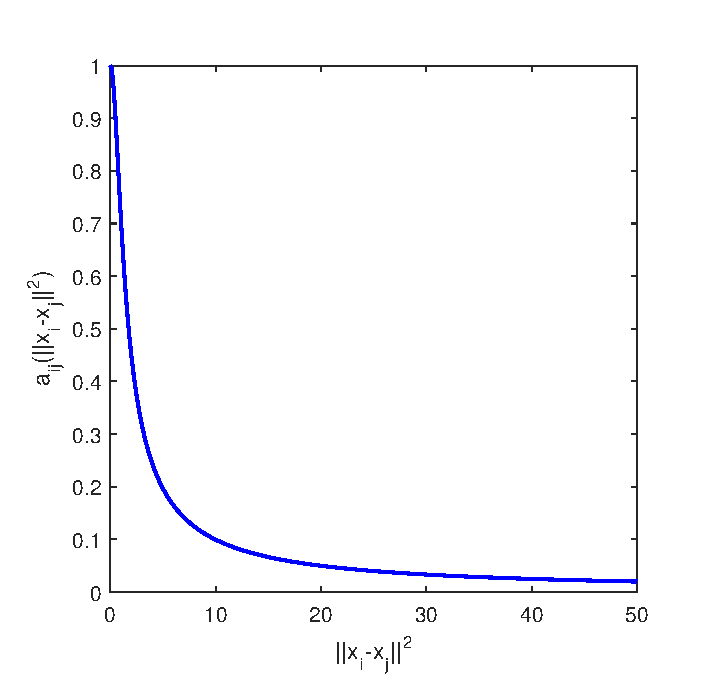
\includegraphics[width=0.32\textwidth]{figure/chapter_2/cs_aij.eps}}
  \subfigure[$f(x)$ with $d_0=1$ and $\theta=2$ in ~\cite{CuckerDong2010}, dashed line represents $x=1$.]{\label{fig:dong_f}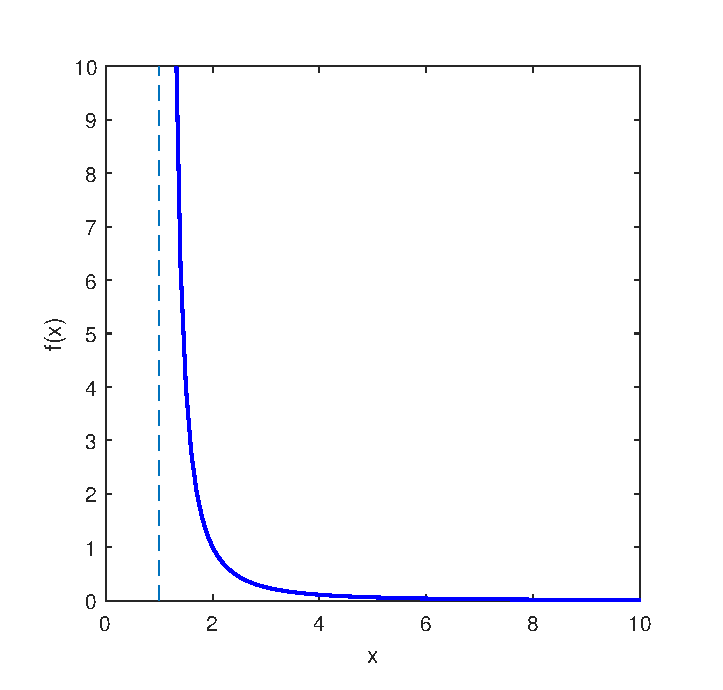
\includegraphics[width=0.32\textwidth]{figure/chapter_2/dong_f.eps}}
  \subfigure[$V_{ij}(x)=\frac{1}{x}+log(x)$, dashed line indicates the global minimum.]{\label{fig:V_ij}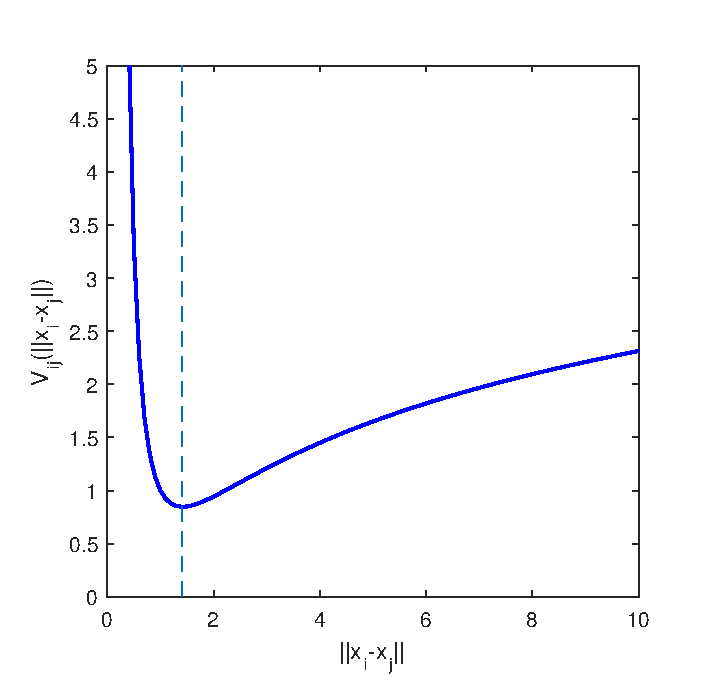
\includegraphics[width=0.32\textwidth]{figure/chapter_2/Vij.eps}}
  \caption{Examples of $a_{ij}(x)$ in~\cite{CuckerSmale2007}, $f(x)$ in~\cite{CuckerDong2010} and $V_{ij}(x)$ in~\cite{FixedTopology}.}\label{fig:example_v}
\end{figure}

\begin{equation}\label{eq:dong_aij}
\begin{aligned}
\ddot{x}_i(t)&=\underbrace{\sum^k_{j=1}a_{ij}(x)(v_j-v_i)}_{\text{velocity consensus term}}+\underbrace{\Lambda(v)\sum_{j\neq i}f(||x_i-x_j||^2)(x_i-x_j)}_{\text{collision avoidance term}}\\
\Lambda(v)&=(\frac{1}{k}\sum_{i>j}||v_i-v_j||^2)^{\frac{1}{2}}
\end{aligned}
\end{equation}

Gradient-based schemes (\ref{eq:fix_topo}) have also been developed in~\cite{FixedTopology,Saber2004,tanner2007flocking,olfati2002distributed} to stabilize inter-agent distances. With the designed artificial potential function $V_{ij}(x)$ (Fig.~\ref{fig:V_ij}) in~\cite{FixedTopology}, the relative distance between agents is expected to locate at the unique minimum. In~\cite{Saber2004}, three flocking rules from~\cite{Reynolds1987}, split, rejoin and squeeze maneuvers have been embodied within their proposed model (\ref{eq:saber}), where $\phi(\cdot)$ is a potential function, $n_{ij}$ is the unit vector along the line connecting $x_i$ and $x_j$ and $a_{ij}$ denotes corresponding adjacency matrix element. When the total number of agents is greater than ten, however, fragmentation may occur that a collective reference pair $(x_r, v_r)$ has to be introduced.

\begin{equation}\label{eq:fix_topo}
\ddot{x}_i(t)=\underbrace{\sum_{j\in V}(v_j-v_i)}_{\text{velocity consensus term}}+\underbrace{(-\sum_{j\in V}\bigtriangledown_{x_i}V_{ij})}_{\text{gradient-based term}}
\end{equation}

\begin{equation}\label{eq:saber}
\ddot{x}_i(t)=\underbrace{\sum_{j\in V}a_{ij}(x)(v_j-v_i)}_{\text{velocity consensus term}}+\underbrace{\sum_{j\in V}\phi(||x_j-x_i||_{\sigma})n_{ij}}_{\text{gradient-based term}}+\underbrace{(-c_1(x_i-x_r)-c_2(v_i-v_r))}_{\text{navigational feedback term}}
\end{equation}

\subsection{First-Order System}

In~\cite{Stability} (\ref{eq:att_rep}),~\cite{Connectedness} (\ref{eq:connect}) and~\cite{Invariant} (\ref{eq:unbound}), first-order control models have been studied that with carefully designed attraction and repulsion functions, Lyapunov function candidates and LaSalle's Invariant Principle, all the flock members are expected to converge to a constant arrangement ($\dot{\mathbf{x}}=0$) within a hyper-ball. Separation is ensured in the first-order system, however, velocity alignment is less satisfied.

\begin{equation}\label{eq:att_rep}
\dot{x}_i=\sum^N_{j=1}(1-e^{-||x_i-x_j||^2})(x_j-x_i)
\end{equation}

\begin{equation}\label{eq:connect}
\dot{x}_i=-\sum_{j\in V}\frac{\partial W_{ij}}{\partial x_i}-\sum_{j\in V}\frac{\partial V_{ij}}{\partial x_i}
\end{equation}

\begin{equation}\label{eq:unbound}
\dot{x}_i=\sum_{j\in V}\frac{2\rho_{ij}}{\gamma_{ij}^2}(D_{ij})_i\mathbf{x}
\end{equation}

\section{Dynamic Topology}

Unlike above mentioned theories assume,~\cite{PNAS} discovered that interaction between agents in flocking does not necessarily depend on the metric distance but rather on the topological distance. An average number of six to seven nearest neighbors are involved in the interaction instead of the whole neighbors within a fixed distance. An example is illustrated in Fig.~\ref{fig:knn}, where the number of nearest neighbors involved, denoted by $q$, is three and the total number of agents, denoted by $k$, is six. Given conditional initial positions, velocities and original $a_{ij}$ in (\ref{eq:vicsek_aij}),~\cite{KNN} has proved that the agents asymptotically agree on a common velocity. Based on~\cite{KNN},~\cite{CuckerDong2016} have further introduced the quotient $\frac{q}{k-1}$ that unconditional flocking occurs when $\frac{q}{k-1}\geq\frac{1}{2}$.

In~\cite{DynamicTopology}, it is shown that with modified potential function (Fig.~\ref{fig:U_ij}), where the potential is constant when the relative distance between two agents is larger than a certain limit and original control model (\ref{eq:fix_topo}), the stability of the flock is guaranteed if no agent is separated initially.

\begin{figure}[H]
  \centering
  \subfigure[A flock of agents with $q=3, k=6$, three closest neighbors of agent 1 and agent 5 are agents 2, 3 and 6 and agents 1, 4 and 6 respectively.]{\label{fig:knn}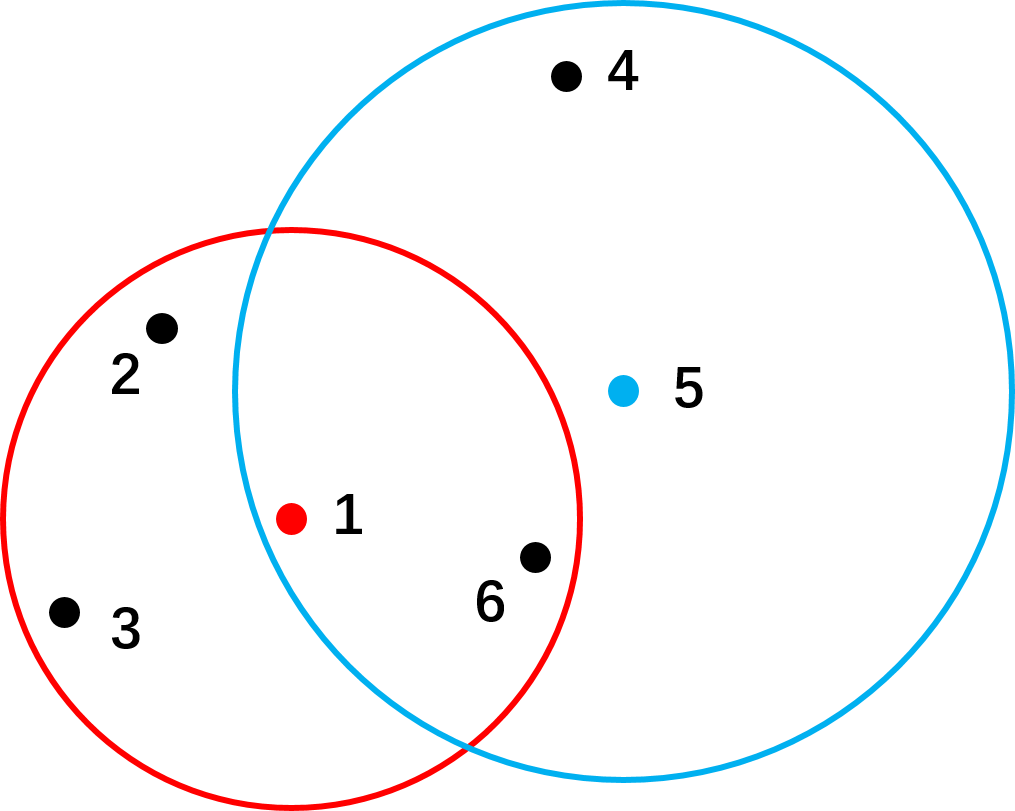
\includegraphics[width=0.4\textwidth]{figure/chapter_2/knn.png}}
  \subfigure[$V_{ij}$ in~\cite{DynamicTopology}. The left dashed line indicates the global minimum and the right dashed line indicates a interaction range. The disconnection of the potential function does not affect the stability.]{\label{fig:U_ij}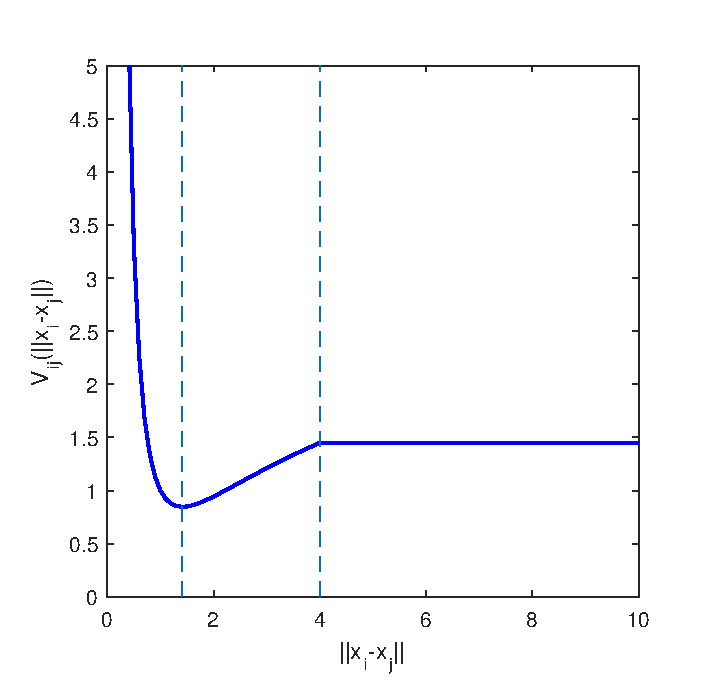
\includegraphics[width=0.4\textwidth]{figure/chapter_2/U.eps}}
  \caption{Examples of dynamic topology and modified potential function.}
\end{figure}

\newpage
